\documentclass[12pt,a4paper]{article}%
%\usepackage{xeCJK}
%\setCJKmainfont{cwTeX Q Yuan Medium}
\usepackage{makeidx}
\makeindex
\usepackage{bm}
\usepackage{framed} % Easier way to use Framebox
\usepackage{pdfpages} % Import PDF in latex document
\usepackage{listings}
\usepackage{array}
\usepackage{enumitem}
\usepackage{amsmath, amssymb, amsthm}  % For mathematical symbols
\usepackage{colortbl,color}
\usepackage{xcolor}
\usepackage{auto-pst-pdf}
\usepackage{graphicx}
\usepackage{psfrag}
\usepackage{multirow}
\usepackage{multicol}
\usepackage{caption}
\usepackage{appendix}
\usepackage{blkarray} %For adding Matrix label on row and column
\usepackage{url}
\usepackage{indentfirst} % indent the first paragraph of new section
\usepackage{titlesec} % change the way \subsubsubsection formats

\def\se{{\rm se}}
%\newcommand{\red}{\color{red}}
\linespread{1.5}  % The linespread is 1.5.

% Numbered theorems, definitions, algorithm and lemmas ======================================================================
\newtheorem{thm}{Theorem}  % Define new theorem.
\newtheorem{alg}{Algorithm}[section]  % Define new algorithm.
\newtheorem{definition}{Definition}
% ===========================================================================================================================

% For writing pseudo code ======================================================================
\usepackage{algorithm}% http://ctan.org/pkg/algorithms
\usepackage{algpseudocode}% http://ctan.org/pkg/algorithmicx
% ===========================================================================================================================

\theoremstyle{definition}
\theoremstyle{plain}
\setcounter{secnumdepth}{5}


\renewcommand{\contentsname}{Table of Contents}
\renewcommand{\listfigurename}{List of Figures}
\renewcommand{\listtablename}{List of Tables}
\renewcommand{\figurename}{Figure}
\renewcommand{\tablename}{Table}
\newcommand{\loflabel}{Figure}
\newcommand{\lotlabel}{Table}
\setlength{\abovecaptionskip}{0pt}


\renewcommand{\appendixpagename}{\Large Appendix} % \ctxfb
\renewcommand{\arraystretch}{1.2}

\usepackage{appendix}


\newtheorem{lma}{\textbf{Lemma}}
% ======================== Set length ========================
\setlength{\columnsep}{1cm}
\setlength\parindent{0pt}
\textheight = 22cm
\textwidth = 16.5cm
\hoffset=-1cm
\footskip=40pt
\renewcommand*{\arraystretch}{0.8}
% ============================================================
% ======================== Paragraph Indent ========================
\setlength{\parindent}{1em}
\setlength{\parskip}{1em}
% ==================================================================
% =============================
% Equation numbering
\numberwithin{equation}{section}
% =============================
% ======================== SubSubSubSection Format ========================
\titleclass{\subsubsubsection}{straight}[\subsection]

\newcounter{subsubsubsection}[subsubsection]
\renewcommand\thesubsubsubsection{\thesubsubsection.\arabic{subsubsubsection}}

\titleformat{\subsubsubsection}
  {\normalfont\normalsize\bfseries}{\thesubsubsubsection}{1em}{}
\titlespacing*{\subsubsubsection}
{0pt}{3.25ex plus 1ex minus .2ex}{1.5ex plus .2ex}
% ==================================================================

\begin{document}
\section{April 23}
\subsection{How to adjust Learning Rate}

Assume the objective function,
\begin{equation}
\underset{\theta}{\text{minimize}}~~ f(\theta) = 0.5(\theta_{1}^{2}-\theta_{2})^{2} + 0.5(\theta_{1}-1)^{2}
\end{equation}

where $\theta$ includes $\theta_{1}$ and $\theta_{2}$.

The figure for the 2D model looks like,
\begin{figure}[H]
\centering
\psfrag{x}{$\theta_{1}$}
\psfrag{y}{$\theta_{2}$}
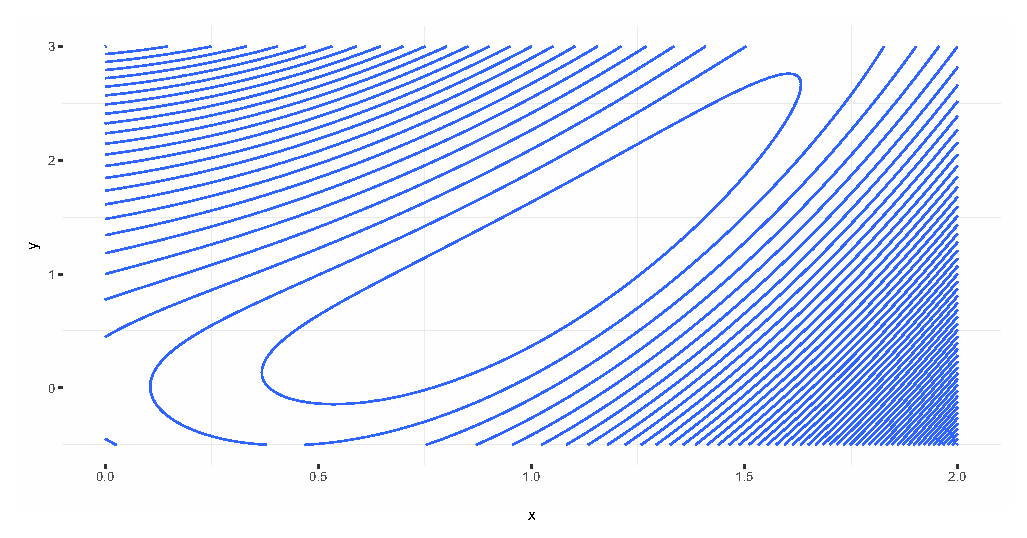
\includegraphics[scale=0.8]{images//plot.eps}
\\~\\
\end{figure}


Next, in order to update $\theta$, we should find the gradients for both $\theta_{1},\theta_{2}$, 
\begin{align*}
\frac{\partial}{\partial \theta_{1}}f(\theta) &= 2\theta_{1}^{3} - 2 \theta_{1} \theta_{2} + \theta_{1} -1 \\
\frac{\partial}{\partial \theta_{2}}f(\theta) &=  - \theta_{1}^{2} + \theta_{2} \\
\end{align*}

Therefore, the update of $\theta$ takes the form,
\begin{align*}
\theta_{1}^{(n+1)} &= \theta_{1}^{(n)} - \alpha_{1} \frac{\partial}{\partial \theta_{1}^{(n)}}f(\theta)= \theta_{1}^{(n)} - \alpha_{1} \big( 2(\theta_{1}^{(n)})^{3} - 2 \theta_{1}^{(n)} \theta_{2}^{(n)} + \theta_{1}^{(n)} -1 \big)   \\
\theta_{2}^{(n+1)} &= \theta_{2}^{(n)} - \alpha_{2} \frac{\partial}{\partial \theta_{2}^{(n)}}f(\theta)= \theta_{2}^{(n)} - \alpha_{2} \big( - (\theta_{1}^{(n)})^{2} + \theta_{2}^{(n)} \big)
\end{align*}

From the definition of fixed point theory, which given a function $f$ defined on the real numbers with real values and given a point $x_{0}$ in the domain of $f$, the fixed point iteration is
\begin{equation}
x_{n+1} = f(x_{n}), n=0,1,\dots
\end{equation}
which gives rise to the sequence $x_{0},x_{1},\dots$, which is hoped to converge to a point $x$. 


By implementing fixed point iteration in our update model, we hope  $\theta^{(0)},\theta^{(1)},\dots$ at any iteration (Superscript indicates iteration) will converge to a point $\theta$
\begin{align*}
\theta_{1}^{(n+1)} &=  f(\theta_{1}^{(n)}) \rightarrow \theta_{1}^{*} =  f(\theta_{1}^{*}) \\
\theta_{2}^{(n+1)} &=  f(\theta_{2}^{(n)}) \rightarrow \theta_{2}^{*} =  f(\theta_{2}^{*})
\end{align*}

By applying Taylor series, we can approximate $f(\theta^{*})$
\begin{equation*}
f(\theta^{*}) = f'(\theta^{*}) |\theta^{(n)}-\theta^{*}|
\end{equation*}

We hope $0<|f'(\theta^{*})|<1$, so $f(\theta^{*})$ will converge. Following the definitions defined above, we derived the range for the learning rate $\alpha_{1}$, 
\begin{equation*}
\frac{\partial}{\partial \theta_{1}^{*}}f(\theta_{1}^{*}) = 1 - \alpha_{1} (6\big(\theta_{1}^{*})^{2} - 2 \theta_{2}^{*}+1 \big)
\end{equation*}

Lower Bound : $0<|f'(\theta_{1}^{*})|$ , 
\begin{align*}
0 &< 1 - \alpha_{1} \big(6(\theta_{1}^{*})^{2} - 2 \theta_{2}^{*}+1 \big) \\
\alpha_{1} &< \frac{1}{6(\theta_{1}^{*})^{2} - 2 \theta_{2}^{*}+1}
\end{align*}


Upper Bound : $|f'(\theta_{1}^{*})|<1$ , 
\begin{align*}
-1 &< 1 - \alpha_{1} \big(6(\theta_{1}^{*})^{2} - 2 \theta_{2}^{*}+1 \big) < 1 \\
0 &< \alpha_{1} < \frac{2}{6(\theta_{1}^{*})^{2} - 2 \theta_{2}^{*}+1}
\end{align*}

$\alpha_{1}$ boundary,
\begin{equation*}
0 < \alpha_{1} < \frac{1}{6(\theta_{1}^{*})^{2} - 2 \theta_{2}^{*}+1}
\end{equation*}

%=============================
Following the same logic, we derive the bellow formula to extract the range for the learning rate $\alpha_{2}$, 
\begin{equation*}
\frac{\partial}{\partial \theta_{2}^{*}}f(\theta_{2}^{*}) = 1 - \alpha_{2}
\end{equation*}

Lower Bound : $0<|f'(\theta_{2}^{*})|$ , 
\begin{align*}
0 &< 1-\alpha_{2} \\
\alpha_{2} &< 1
\end{align*}


Upper Bound : $|f'(\theta_{2}^{*})|<1$ , 
\begin{align*}
-1 &< 1-\alpha_{2} < 1 \\
0 &< \alpha_{2} < 2
\end{align*}

$\alpha_{2}$ boundary,
\begin{equation*}
0 < \alpha_{1} < 1
\end{equation*}

Applying the learning rate $\alpha_{1} = \frac{1}{6(\theta_{1}^{*})^{2} - 2 \theta_{2}^{*}+1}$ and $\alpha_{2} = 1 $. The searching path,

\begin{figure}[H]
\centering
\psfrag{x}{$\theta_{1}$}
\psfrag{y}{$\theta_{2}$}
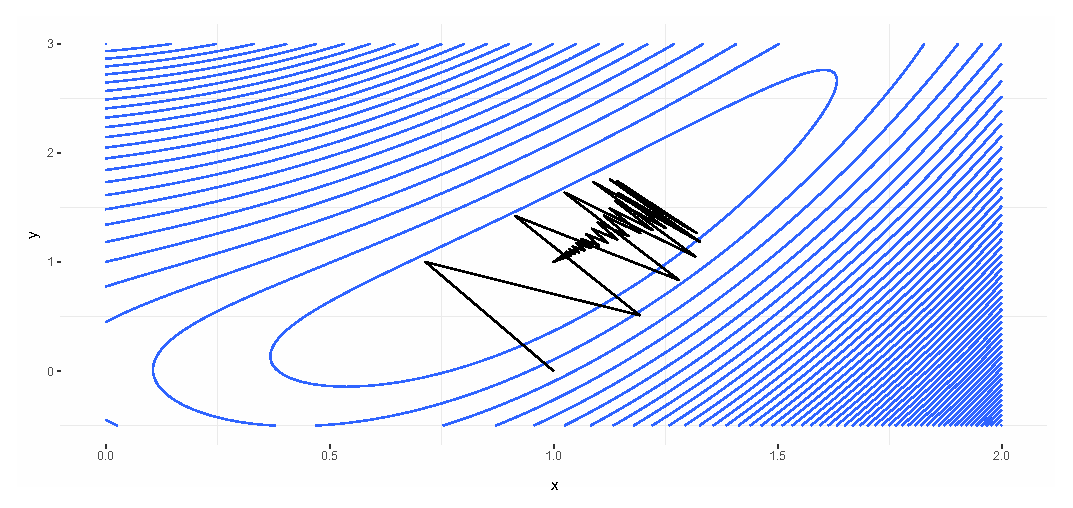
\includegraphics[scale=0.8]{images//searching.eps}
\\~\\
\end{figure}

\textbf{R code:}
\tiny
\begin{lstlisting}[language=R]
library(ggplot2)

mytheme = theme_bw() + theme(panel.border = element_blank(), panel.grid.major = element_blank())

theta1_seq <- seq(0, 2,length.out =  1000)
theta2_seq <- seq(-0.5,3,length.out =  1000)
data = expand.grid(x = theta1_seq,y = theta2_seq,KEEP.OUT.ATTRS = FALSE)


response = function(theta1,theta2){
  return(0.5*(theta1^2-theta2)^2+0.5*(theta1-1)^2)
}

data = cbind(data, response = response(data$x,data$y))

plot = ggplot(data, aes(x = x, y = y, z=response)) + stat_contour(binwidth = 0.2)+mytheme


searching = data.frame(theta1=rep(0,100),theta2=rep(0,100),response=rep(0,100))

theta1 = 0
theta2 = 0

for(i in 1:100){
  theta1_new = theta1 - ((1/((6*(theta1^{2}))-(2*theta2)+1)))*(2*theta1^{3}-2*theta1*theta2+theta1-1)
  theta2_new = theta2 - (1)*(-(theta1^2)+theta2)
  response_value = response(theta1_new,theta2_new)
  
  theta1 = theta1_new
  theta2 = theta2_new
  
  cat("Iteration:", i,"\n")
  cat("theta1: ", theta1, "\n")
  cat("theta2: ", theta2, "\n")
  cat("Response: ", response_value,"\n")
  searching[i,1] = theta1
  searching[i,2] = theta2
  searching[i,3] = response_value
}

plot + geom_path(data=searching, aes(x=theta1,y=theta2))

\end{lstlisting}

\end{document}
